\documentclass[titlepage]{article}
\usepackage{babel}
\usepackage{amsmath}
\usepackage{amssymb}
\usepackage{amsthm}
\usepackage{multicol} %spalten in seite
\usepackage{graphicx} %bilder einfügen
\usepackage[normalem]{ulem} %durchstreichen
\usepackage{tabto} %tabulator mit \tab
\usepackage{hyperref}
\usepackage{tikz}
\usetikzlibrary{shapes.geometric}
\usepackage{wasysym}
\usepackage{bbm}
\usepackage{bbold}
\usepackage{xcolor}
\usepackage[T1]{fontenc}
\usepackage{mathrsfs}  
\usepackage[utf8]{inputenc}
\usepackage{listings} %quellcode
\pagestyle{plain}
\pagenumbering{arabic}
\renewcommand{\arraystretch}{1.3} %vertikaler abstand von tabellen
\newcommand{\n}{\newline}
\usepackage[left=20mm, right=15mm, top=25mm, bottom=7mm, paper=a4paper]{geometry}

\renewcommand{\contentsname}{Inhaltsverzeichnis}
\newcommand{\K}{\mathbb{K}}
\newcommand{\C}{\mathbb{C}}
\newcommand{\N}{\mathbb{N}}
\newcommand{\Q}{\mathbb{Q}}
\newcommand{\R}{\mathbb{R}}
\newcommand{\1}{\mathbb{1}}
\newcommand{\0}{\mathbb{0}}
\newcommand{\Z}{\mathbb{Z}}
\newcommand{\vecV}[4]{\left(\begin{smallmatrix}#1\\#2\\#3\\#4\end{smallmatrix}\right)}
\newcommand{\smallMatrixD}[9]{\left(\begin{smallmatrix}#1&#2&#3\\#4&#5&#6\\#7&#8&#9\end{smallmatrix}\right)}
\newcommand{\la}{\langle}
\newcommand{\ra}{\rangle}
\newcommand{\vecD}[3]{\left(\begin{smallmatrix}#1\\#2\\#3\end{smallmatrix}\right)}
\newcommand{\matrixZ}[4]{\begin{pmatrix}#1&#2\\#3&#4\end{pmatrix}}
\newcommand{\detZ}[4]{\begin{vmatrix}#1&#2\\#3&#4\end{vmatrix}}
\newcommand{\smallMatrixZ}[4]{\left(\begin{smallmatrix}#1&#2\\#3&#4\end{smallmatrix}\right)}
\newcommand{\smallDetZ}[4]{\left|\begin{smallmatrix}#1&#2\\#3&#4\end{smallmatrix}\right|}
\newcommand{\vecZ}[2]{\left(\begin{smallmatrix}#1\\#2\end{smallmatrix}\right)}
\newcommand{\detD}[9]{\begin{vmatrix}#1&#2&#3\\#4&#5&#6\\#7&#8&#9\end{vmatrix}}
\newcommand{\matrixD}[9]{\begin{pmatrix}#1&#2&#3\\#4&#5&#6\\#7&#8&#9\end{pmatrix}}
\newcommand{\skalarProdukt}[2]{\langle#1\mid#2\rangle}
\newcommand{\sarrusD}[9]{(#1)\cdot(#5)\cdot(#9)+(#4)\cdot(#8)\cdot(#3)+(#7)\cdot(#2)\cdot(#6)-(#7)\cdot(#5)\cdot(#3)-(#1)\cdot(#8)\cdot(#6)-(#4)\cdot(#2)\cdot(#9)}
\newcommand{\kreuzproduktD}[6]{\left(\begin{matrix}#2#6-#3#5\\#3#4-#1#6\\#1#5-#2#4\end{matrix}\right)}

\begin{document}
	
	\begin{center}
		
\begin{tikzpicture}
			\draw (0,0) node[draw, rectangle]{\textsc{Wintersemester 2020/21}};
		\end{tikzpicture}
		\hrulefill\\
		\begin{center}
			\LARGE\textsc{Lineare Algebra - Übung 12} \normalsize\\
		\end{center}
		\hrulefill
		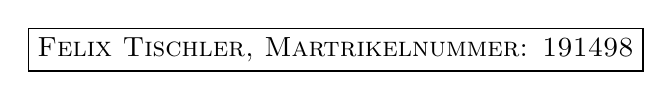
\begin{tikzpicture}
			\draw (0,0) node[draw, rectangle]{\textsc{Felix Tischler, Martrikelnummer: 191498}};
		\end{tikzpicture}
		\date{\today}
	\end{center}

	%\part*{Hausaufgaben (Abgabe bis 08.02.2021, 14:00 Uhr)}
	\paragraph{Hausaufgabe 12.1:} \textit{Orthogonales Komplement} \\ Sei $(V,\la\mid\ra)$ ein Skalarproduktraum und $M\subseteq V.$ \\
	\begin{proof}[a) Beweis:]
		$M^{\perp}=\{\vec{v}\in V\mid\forall\vec{u}\in M:\vec{v}\perp\vec{u}\}\subseteq V$: \\\\ \indent 1) $\vec{0}\in V\Rightarrow\vec{0}\in M^{\perp}$. \\\\ \indent 2) Sei $\lambda,\mu\in\R$ und $\vec{u},\vec{v}\in M^{\perp}$. \\\\ \indent\quad\quad Zz.: $\lambda\vec{u}+\mu\vec{v}\in M^{\perp}\Leftrightarrow\forall\vec{m}\in M:(\lambda\vec{u}+\mu\vec{v})\perp\vec{m}\Leftrightarrow\forall\vec{m}\in M:\la\lambda\vec{u}+\mu\vec{v}\mid\vec{m}\ra=0$. \\\\ \indent\quad\quad $\la\lambda\vec{u}+\mu\vec{v}\mid\vec{m}\ra=\lambda\underbrace{\la\vec{u}\mid\vec{m}\ra}_0+\mu\underbrace{\la\vec{v}\mid\vec{m}\ra}_0=\lambda\cdot0+\mu\cdot0=0.$
	\end{proof}
	\noindent
	\begin{proof}[b) Beweis:]
		$\forall\vec{m}\in M:\vec{m}$ ist zu allen $\vec{v}\in M^\perp$ orthogonal $\Rightarrow\vec{m}\in(M^\perp)^\perp\Rightarrow M\subseteq(M^\perp)^\perp$
	\end{proof}
	\noindent
	\textit{c)} Berechnung: $\{u\}^\perp=\{\vec{v}\in V\mid \vec{v}\perp\vec{u}\}=\{\vec{v}\in V\mid\la\vec{v}\mid\vec{u}\ra=0\}$
	\begin{align*}
		\la\vecD{x}{y}{z}\mid\vecD{1}{-2}{2}\ra\overset{!}{=}0\Leftrightarrow x\cdot1+y\cdot(-2)+z\cdot2\overset{!}{=}0\Rightarrow x=2y-2z,y=y,z=z\Rightarrow \{\vec{u}\}^\perp=Span(\vecD{2}{1}{0},\vecD{-2}{0}{1})
	\end{align*}

	\paragraph{Hausaufgabe 12.2:} \textit{Orthonormalisierung} \\ Sei $[\vec{u}_1,\dots,\vec{u}_4]\subset\R^4,\vec{u}_1:=\vecV{2/3}{-2/3}{0}{1/3},\vec{u}_2:=\vecV{-2/3}{-2/3}{1/3}{0},\vec{u}_3:=\vecV{0}{1}{0}{0},\vec{u}_4:=\vecV{0}{0}{0}{1}.$
	\\ Orthogonalisierung:
	\begin{align*}
		\vec{w}_1&=\vec{u}_1\textit{ und }\skalarProdukt{\vec{w}_1}{\vec{w}_1}=(4/9)+(4/9)+(1/9)=1
		\\\\
		\vec{w}_2&=\vec{u}_2-\frac{\skalarProdukt{\vec{u}_2}{\vec{w}_1}}{\skalarProdukt{\vec{w}_1}{\vec{w}_1}}\cdot\vec{w}_1
		=\vecV{-2/3}{-2/3}{1/3}{0}-\frac{(-4/9)+(4/9)}{1}\cdot\vecV{2/3}{-2/3}{0}{1/3}=\vec{u}_2\\
		&\textit{ und }\skalarProdukt{\vec{w}_2}{\vec{w}_2}=(4/9)+(4/9)+(1/9)=1
		\\\\
		\vec{w}_3&=\vec{u}_3-\frac{\skalarProdukt{\vec{u}_3}{\vec{w}_1}}{\skalarProdukt{\vec{w}_1}{\vec{w}_1}}\cdot\vec{w}_1-\frac{\skalarProdukt{\vec{u}_3}{\vec{w}_2}}{\skalarProdukt{\vec{w}_2}{\vec{w}_2}}\cdot\vec{w}_2
		=\vecV{0}{1}{0}{0}+\frac{2/3}{1}\cdot\vecV{2/3}{-2/3}{0}{1/3}+\frac{2/3}{1}\cdot\vecV{-2/3}{-2/3}{1/3}{0}=\vecV{0}{1/9}{2/9}{2/9}\\
		&\textit{ und }\skalarProdukt{\vec{w}_3}{\vec{w}_3}=\frac{1}{81}+\frac{4}{81}+\frac{4}{81}=\frac{9}{81}=\frac{1}{9}
		\\\\
		\vec{w}_4&=\vec{u}_4-\frac{\skalarProdukt{\vec{u}_4}{\vec{w}_1}}{\skalarProdukt{\vec{w}_1}{\vec{w}_1}}\cdot\vec{w}_1-\frac{\skalarProdukt{\vec{u}_4}{\vec{w}_2}}{\skalarProdukt{\vec{w}_2}{\vec{w}_2}}\cdot\vec{w}_2-\frac{\skalarProdukt{\vec{u}_4}{\vec{w}_3}}{\skalarProdukt{\vec{w_3}}{\vec{w}_3}}\cdot\vec{w}_3
		\\
		&=\vecV{0}{0}{0}{1}-\frac{1/3}{1}\cdot\vecV{2/3}{-2/3}{0}{1/3}-\frac{0}{1}\cdot\vecV{-2/3}{-2/3}{1/3}{0}-\frac{2/9}{1/9}\cdot\vecV{0}{1/9}{2/9}{2/9}=\vecV{0}{0}{0}{1}-\vecV{2/9}{-2/9}{0}{1/9}-\vecV{0}{2/9}{4/9}{4/9}=\vecV{-2/9}{0}{-4/9}{4/9}
	\end{align*}
	\\ Normalisierung:
	\begin{align*}
		&\vec{w}_1=\vecV{2/3}{-2/3}{0}{1/3},\vec{w}_2=\vecV{-2/3}{-2/3}{1/3}{0},\vec{w}_3=\vecV{0}{1/9}{2/9}{2/9},\vec{w}_4=\vecV{-2/9}{0}{-4/9}{4/9}\textit{ und }\vec{v}_r=\frac{\vec{w}_r}{||\vec{w}_r||}\\
		&||\vec{w}_1||=||\vec{w}_2||=1\\
		&||\vec{w}_3||=\sqrt{(1/81)+(4/81)+(4/81)}=\sqrt{1/9}=\frac{1}{3}\Rightarrow\vec{w}_3=3\cdot\vecV{0}{1/9}{2/9}{2/9}=\vecV{0}{1/3}{2/3}{2/3}\\
		&||\vec{w}_4||=\sqrt{(4/81)+(16/81)+(16/81)}=\sqrt{36/81}=\sqrt{4/9}=\frac{2}{3}\Rightarrow\vec{w}_4=\frac{3}{2}\cdot\vecV{-2/9}{0}{-4/9}{4/9}=\vecV{-1/3}{0}{-2/3}{2/3}
	\end{align*}
	D.h. $\vec{w}_1=\vecV{2/3}{-2/3}{0}{1/3},\vec{w}_2=\vecV{-2/3}{-2/3}{1/3}{0},\vec{w}_3=\vecV{0}{1/3}{2/3}{2/3},\vec{w}_4=\vecV{-1/3}{0}{-2/3}{2/3}$
	
	\paragraph{Hausaufgabe 12.3:} \textit{Hauptachsentransformation} \\ Sei $A:=\smallMatrixD{1}{-1}{-2}{-1}{1}{-2}{-2}{-2}{-2}\in M_3(\R).$\\\\
	Eigenwerte:
	\begin{align*}
		\detD{X-1}{1}{2}{1}{X-1}{2}{2}{2}{X+2}&\overset{(1)}{=}\detD{X-2}{1}{2}{0}{X-1}{2}{(-X/2)+1}{2}{X+2}\overset{(2)}{=}\detD{X-2}{1}{2}{0}{X-1}{2}{0}{5/2}{X+3}\overset{(3)}{=}(X-2)\cdot\detZ{X-1}{2}{5/2}{X+3}\\
		&\overset{(4)}{=}(X-2)(X^2+2X-8)\Rightarrow X_1=2,X_2=-1+\sqrt{9}=2,X_3=-1-\sqrt{9}=-4
	\end{align*}
	\begin{enumerate}
		\item[(1)] Spalte I minus $\frac{1}{2}$ Spalte III
		\item[(2)] Zeile III plus $\frac{1}{2}$ Zeile I
		\item[(3)] Laplace nach Spalte I
		\item[(4)] Sarrus
	\end{enumerate}
	Eigenvektoren:
	\begin{align*}
		&\lambda_{1,2}: & &\lambda_3:\\
		&\matrixD{1}{1}{2}{1}{1}{2}{2}{2}{4}\Rightarrow Span(\vecD{-2}{0}{1},\vecD{-1}{1}{0}) & &\matrixD{-5}{1}{2}{1}{-5}{2}{2}{2}{-2}\Rightarrow Span(\vecD{1}{1}{2})
	\end{align*}
	\noindent
	Gram-Schmidt Verfahren:
	\begin{align*}
		&\lambda_{1,2}: & &\lambda_3:\\
		&\vec{u}_1=\vecD{-2}{0}{1},\vec{u}_2=\vecD{-1}{1}{0} & &\vec{u}_3=\vecD{1}{1}{2}\\
		&\vec{w}_1=\vec{u}_1,\vec{w}_2=\vec{u}_2-\frac{\skalarProdukt{\vec{u}_2}{\vec{w}_1}}{\skalarProdukt{\vec{w}_1}{\vec{w}_1}}\cdot\vec{w}_1 & &\vec{w}_3=\vec{u}_3\\
		&\vec{w}_2=\vecD{-1}{1}{0}-\frac{2}{5}\cdot\vecD{-2}{0}{1}=\vecD{-1/5}{1}{-2/5} & &||\vec{w}_3||=\sqrt{6}\Rightarrow\vec{w}_3=\frac{1}{\sqrt{6}}\vecD{1}{1}{2}=\vecD{1/\sqrt{6}}{1/\sqrt{6}}{2/\sqrt{6}}\\
		&||\vec{w}_1||=\sqrt{5}\Rightarrow\vec{w}_1=\frac{1}{\sqrt{5}}\vecD{-2}{0}{1}=\vecD{-2/\sqrt{5}}{0}{1/\sqrt{5}} &&\\
		&||\vec{w}_2||=\sqrt{6/5}\Rightarrow\vec{w}_2=\frac{1}{\sqrt{6/5}}\vecD{-1/5}{1}{-2/5}=\vecD{-\sqrt{30}}{1/\sqrt{6/5}}{-\sqrt{30}/15}
	\end{align*}
	Aus den Ergebnissen des Gram-Schmidt Verfahrens folgt $S=(\vec{w}_1,\vec{w}_2,\vec{w}_3)$:
	\begin{align*}
		S=\matrixD{-2/\sqrt{5}}{-\sqrt{30}/30}{1/\sqrt{6}}{0}{1/\sqrt{6/5}}{1/\sqrt{6}}{1/\sqrt{5}}{-\sqrt{30}/15}{2/\sqrt{6}}\textit{ und }\detD{-2/\sqrt{5}}{-\sqrt{30}/30}{1/\sqrt{6}}{0}{1/\sqrt{6/5}}{1/\sqrt{6}}{1/\sqrt{5}}{-\sqrt{30}/15}{2/\sqrt{6}}=-1
	\end{align*}
	Da $det(S)=-1$ folgt $\tilde{S}=(-\vec{w}_1,\vec{w}_2,\vec{w}_3)$. 
	
	\paragraph{Anmerkung:} Die Berechnung von $det(S)$ hab ich hier noch ergänzt:
	\begin{align*}
		det(S)&=\detD{-2/\sqrt{5}}{-\sqrt{30}/30}{1/\sqrt{6}}{0}{1/\sqrt{6/5}}{1/\sqrt{6}}{1/\sqrt{5}}{-\sqrt{30}/15}{2/\sqrt{6}}\overset{(1)}{=}\detD{-2/\sqrt{5}}{-\sqrt{30}/30}{1/\sqrt{6}}{0}{1/\sqrt{6/5}}{1/\sqrt{6}}{0}{-\sqrt{30}/12}{5/2\sqrt{6}}\overset{(2)}{=}-\frac{2}{\sqrt{5}}\detZ{1/\sqrt{6/5}}{1/\sqrt{6}}{-\sqrt{30}/12}{5/2\sqrt{6}}\\
		&\overset{Sarrus}{\Rightarrow}-\frac{2}{\sqrt{5}}\left[\left(\frac{1}{\sqrt{6/5}}\cdot\frac{5}{2\sqrt{6}}\right)+\left(\frac{\sqrt{30}}{12}\cdot\frac{1}{\sqrt{6}}\right)\right]=-\frac{2}{\sqrt{5}}\left(\frac{5\sqrt{5}}{12}+\frac{\sqrt{5}}{12}\right)=-\frac{12\sqrt{5}}{12\sqrt{5}}=-1
	\end{align*}
	\begin{enumerate}
		\item[(1)] III+$\frac{1}{2}$I
		\item[(2)] Laplace nach Spalte I
	\end{enumerate}
\end{document}
